\chapter{Implementacja symulatora}

\par{
W poprzednich rozdziałach opisano generalne zasady wg. których powinien funkcjonować symulator środowiska miejskiego przystosowany do współpracy z systemem fuzji danych. Wskazano czym powinien się cechować by dobrze spełniać stawiane przed nim zadania - w szczególności być w stanie zapewnić dane użyteczne z punktu widzenia prowadzenia badań nad systemem fuzji danych.
}
\par{
W tym rozdziale zostanie omówiona implementacja takiego symulatora by pokazać jak w praktyce można spełnić wymagania stawiane tego rodzaju aplikacjom, jakie problemy mogą zostać napotkane i jak można sobie z nimi radzić a także jakiego rodzaju technologie można zastosować do uzyskania określonych celów.
}
\par{
W dalszej części rozdziału zostaną omówione ograniczenia tego rodzaju symulacji ze szczególnym uwzględnieniem ograniczeń wydajnościowych. Autor postara się zwrócić uwagę na największe ograniczenia takich systemów - czyli miejsca potencjalnej optymalizacji. Jednocześnie wskazane będą miejsca, które choć mogą wydawać się krytyczne z punktu widzenia symulacji przy konieczności współpracy z systemem fuzji danych przestają w ogóle odgrywać rolę, przynajmniej z punktu widzenia wydajności.
}

\section[Wymagania][Wymagania]{Wymagania}

\par{
Tak jak i inne systemy informatyczne tak i ten, choć projektowany w ramach pracy inżynierskiej musiał spełniać pewne wymagania wynikające z możliwości jego późniejszego zastosowania do badań naukowych a w szczególności do pracy Pana Macieja Grzybka dotyczącej śledzenia obiektów w systemie fuzji danych (temat pracy: "Implementacja algorytmu śledzenia obiektów w systemie fuzji danych").
}
\par{
Poniżej opisano postawione systemowi wymagania:
\begin{itemize}
	\item System powinien dostarczać informacje z czujników w mieście w formie wstępnie przetworzonej (na potrzeby fuzji informacji[?]).
	\item System powinien posiadać przynajmniej jeden typ czujnika, który dostarcza informacji w formie zawierającej co najmniej informację na temat współrzędnych geograficznych obiektu obserwowanego.
	\item System powinien udostępniać odczyty z czujników przy użyciu uzgodnionego schematu bazy danych dynamicznych (podział na bazę statyczną i dynamiczną wyjaśniony w rozdziale "Projekt bazy danych").
	\item System powinien mieć możliwość dodania implementacji bardziej zaawansowanych rodzajów czujników w szczególności posiadających inne właściwości obserwacji, dostarczające innych informacji czy też działające z określonym zaszumieniem.
	\item System powinien prezentować symulację w formie graficznej tak, by można było obserwować jej przebieg i konfrontować go organoleptycznie z wynikami dalszej analizy danych wyjściowych symulacji (ułatwienie dla wstępnej fazy prowadzenia badań).
	\item System powinien operować na danych dotyczących środowiska miejskiego pobranych z odpowiednio zdefiniowanej struktury bazy danych (wczytywanie map).
	\item System powinien umożliwiać regulację natężenia ruchu lub pozwalać na łatwe doimplementowanie tego rodzaju funkcjonalności w przyszłości.
	\item System powinien umożliwiać regulację szybkości symulacji względem czasu rzeczywistego (przyśpieszenie, spowolnienie).
	\item System powinien pozwalać na czasowe wstrzymanie symulacji.
\end{itemize}
}

\section[Metodyka symulacji][Metodyka symulacji]{Metodyka symulacji}
\subsection{Przedmiot symulacji}
\par{
Jak wspomniano w poprzednim rozdziale, dobranie skali integracji symulacji do wybranego zagadnienia jest istotne z punktu widzenia osiągnięcia zamierzonych rezultatów. Wybranie skali zbyt wysokiej ogranicza możliwości zastosowania symulacji i jej rozszerzalność. Wybranie skali zbyt niskiej skutkuje natomiast utrudnieniami implementacyjnymi, wzrostem złożoności obliczeniowej i skomplikowaniem ogólnej zasady działania symulacji bez rekompensaty w postaci użytecznych możliwości.
}
\par{
Dobranie odpowiedniej skali integracji powinno przede wszystkim uwzględniać skalę w jakiej obserwowany będzie symulowany układ, tak by w tej skali zachowywał się on realistycznie z punktu widzenia celu symulacji[?]. I tak w przypadku przedstawianego w pracy symulatora obserwowane obiekty są obserwowane w stosunkowo wysokiej skali integracji - jako samochody, piesi i inne elementy makro-świata.
}
\par{
Mając na względzie te potrzeby wydaje się więc, że można traktować te obiekty jako niepodzielne elementy i nie zagłębiać się w ich wewnętrzną specyfikę. Warto jednak uwzględnić fakt, że decyzja ta może uniemożliwiać lub w znacznym stopniu utrudniać niektóre przyszłe rozszerzenia symulacji. I tak jak nie będzie zapewne stanowiło problemu dodanie do symulacji obsługi zderzeń niesprężystych gdyż ich obsługa nie wymaga zagłębiania się w budowę obiektów, tak obsługa np. aerodynamiki pojazdów może stanowić znaczące utrudnienie implementacyjne. Należy pamiętać, że nie każde obliczenia mikro skali da się przełożyć na wartości w skali makro [?].
}
\par{
Licząc się z wyżej wspomnianymi konsekwencjami podjęto decyzję, by elementy świata rozpatrywać w skali abstrakcyjnych obiektów o nieznanej wewnętrznej budowie. Będąc świadomym, iż przedmiotem naszej symulacji są właśnie obiekty makro-świata zawieszone w czterowymiarowej przestrzeni (przestrzeń i czas) i będąc świadomym ich właściwości można przystąpić do dalszego planowania metodyki symulacji.
}

\subsection{Model symulacji}
\par{
Poprzedni podrozdział uzasadnił dlaczego przy implementacji symulatora zdecydowano się na nie wgłębianie w wewnętrzną strukturę obiektów a jedynie zasymulowanie ich poprawnego z punktu widzenia celu symulacji zachowania w możliwie prosty sposób. Innym problemem z jakim należało sobie poradzić było ustalenia jak przedstawić owe makroskopowe obiekty by zachowywały się one w sposób realistyczny z punktu widzenia informacji istotnych dla obserwatorów.
}
\par{
Z pomocą przy rozwiązaniu tego problemu przychodzi nam teoria symulacji a także podstawy dynamiki Newtona przedstawione w pierwszym rozdziale.
I tak wiemy, że zastosowanie właśnie modelu newtonowskiego do symulowania ruchów obiektów da nam obraz realistyczny z punktu widzenia makro świata.
}
\par{
Podstawowymi wielkościami dynamiki Newtona są siła (F), przyśpieszenie (a) oraz masa (m), połączone wzorem:
\begin{center}
$F = m \times a$
\end{center}
Wzór ten opisuje podstawę ruchu i odnosi się właśnie do obiektów makroskopowych o nieznanej lub nieokreślonej strukturze wewnętrznej opisywanych modelami fizycznymi takimi jak punkt materialny lub bryła sztywna.
}
\par{
Dla ciał opisywanych przy użyciu symulatora również należało znaleźć odpowiedni model fizyczny. Pod uwagę wzięto dwa wyżej wspomniane modele, jako, że zapewniają one realizm symulacji i pozwalają na uwzględnianie licznych czynników zewnętrznych.
}
\par{
Podejście do obiektów symulowanych jak do bryły sztywnej wydaje się być intuicyjne. W naturalny sposób blokuje to możliwość ingerencji w wewnętrzną fizykę ciała, jednocześnie zapewniając wysoki realizm w skali makro.
Takie podejście pozwala na łatwe zasymulowanie wszelkiego rodzaju zdarzeń niesprężystych, także związanych z obrotami, w sposób naturalny ułatwia wykrywanie kolizji i pozwala przewidywać ich przebieg z dużą dokładnością i z zachowaniem wysokiego realizmu.
Niestety model ten ze względu na stopień kompilacji został odrzucony a wybrany został model prostszy - model punktu materialnego.
\par{
Model punktu materialnego pozwala na wykonywanie wszelkich obliczeń na obiektach które nie nawiązują między sobą interakcji równie dobrze jak model bryły sztywnej. Jego niewątpliwą wadą jest to, że w razie pojawienia się potrzeby symulowania zderzeń między obiektami pojawił by się spory narzut na dość sztucznej warstwie abstrakcji, która musiała by powstać by obsłużyć zderzenia w sposób realistyczny (dodać do modelu odpowiednie siły itp.).
Ponadto model ten nie uwzględnia w ogóle obrotów, ponieważ z jego punktu widzenia obiekty w świecie stają się niematerialnymi punktami bez wymiarów.
Największą i przeważającą zaletą tego modelu była jego prostota, która pozwoliła na szybką implemetację wersji symulatora zdolnej spełniać podstawowe powierzone jej zadania. 
}
\par{
W ramach modelu fizyki punktu materialnego przyjęto, że każdy obiekt w świecie stanowi jeden punkt materialny, który w każdej chwili czasu charakteryzuje się następującymi wartościami:
\begin{itemize}
\item Siła (wektor trójwymiarowy) z jaką działa ciało na świat stanowiący inercjalny układ odniesienia rozumiany jako statyczny obiekt o nieskończonych wymiarach, względem, którego przemieszczają się ciała (swoista podstawa układu).
\item Masa ciała
\item Prędkością (wektor trójwymiarowy) z jaką w danej chwili porusza się ciało.
\end{itemize}
Znając te trzy wartości w każdej chwili czasu na podstawie modelu fizycznego można określić położenie obiektu w układzie współrzędnych w każdej chwili czasu.
Warto zwrócić uwagę, że tak jak pierwsze dwa z tych parametrów są właściwościami obiektu tzn. obiekt może je dowolnie zmieniać w czasie, tak prędkość jest wartością wynikającą z dotychczasowej historii danego obiektu i sam obiekt nie jest w stanie wprost zmienić jej wartości (tak jak w rzeczywistości samochód nie może w jednej chwili się zatrzymać, ale może nagle (w modelu przyjęto że nawet w czasie $\Delta t \longrightarrow 0$) zacząć hamować działając z dużą siłą o zwrocie przeciwnym do kierunku jazdy i szybko (ale nie natychmiastowo) wytracić posiadaną prędkość).
}

\subsection{Upływ czasu}
\par{
Ostatnią z punktu widzenia istoty symulacji decyzją jaką należało podjąć było wybranie jednego z dwóch możliwych podejść do symulowania upływu czasu:

\begin{itemize}
\item Obliczenia przy założeniu ciągłości czasu
\item Obliczenia przy założeniu czasu skwantowanego (dyskretnego)
\end{itemize}
}
\par{
Pierwsze z podejść jest bliższe realizmowi (choć w świetle współczesnych badań fizycznych okazuje się, że czas należy rzeczywiście traktować jako parametr zdyskretyzowany, to gęstość jego rzeczywistego "próbkowania" jest tak duża, że nie sposób obsługiwać ją przy użyciu komputera).
Jak wspominano w poprzednim rozdziale, uzyskanie efektu czasu ciągłego sprowadza się do opisania wszystkich elementów symulowanego świata układem równań. W każdej chwili pozycja każdego obiektu może być wyznaczona jako pozycja początkowa przesunięta o wektor wyznaczany z bieżącego równania ruchu danego ciała. Tego rodzaju symulacja zapobiega wszelkiego rodzaju błędom przybliżeń i błędom kwantowania, ma ona jednak inne właściwości, które dyskwalifikują jej użycie.
}
\par{
Warto zwrócić uwagę, że tego typu równania wyznacza się ponownie ilekroć pojawia się jakiegoś rodzaju zdarzenie. Przez zdarzenie rozumie się tutaj wszelkie sytuacje mogące wpływać na stan jakiegokolwiek ciała. I tak podstawowymi zdarzeniami w typowym modelu fizycznym są np. zderzenia dwóch ciał. W wypadku symulacji zdarzenie następuje jednak również wtedy gdy co najmniej jeden z obiektów zechce pod wpływem czynników zewnętrznych zmienić swój stan (tj. siłę lub masę). Niestety wyznaczanie tego rodzaju momentów w czasie wydaje się być zadaniem bardzo trudnym. Po pierwsze nie jesteśmy w stanie przewidzieć w jakich sytuacjach obiekt będzie chciał zmieniać swój stan - musimy więc przenieść tę odpowiedzialność na niego. Po drugie obiekt taki musi w swoisty sposób przewidywać przyszłość by zaplanować zdarzenie - każdy obiekt musi więc mieć pojęcie o całym układzie by być w stanie (i to przy dużym nakładzie obliczeniowym) przewidzieć i zaplanować zdarzenia, które dotyczą jego stanu ruchu.
}
\par{
Rozwiązaniem, które pozwoliło by wdrożyć ideę czasu ciągłego w życie bez konieczności wprowadzania olbrzymiej ilości obliczeń, jest twarde zdefiniowanie w modelu sytuacji w których poszczególne obiekty mogą zmieniać decyzje. Warto jednak zwrócić uwagę, że zmniejsza to decyzyjność pojedynczych jednostek w świecie co obniża realizm ewentualnie wdrożonej sztucznej inteligencji.
}
\par{
Wyżej wspomniane powody sprawiły, iż zdecydowano się na wybranie wariantu symulacji z czasem jako jednostką skwantowaną. W takiej sytuacji każdy kwant jest punktem decyzji dla każdego obiektu a przez okres jego trwania ciała poruszają się ze stałymi parametrami (przyśpieszenie, prędkość).
Takie rozwiązanie posiada szereg wad. Po pierwsze, w przypadku potrzeby zasymulowania kolizji pojawia się problem nachodzenia na siebie obiektów. W typowym przypadku zderzenia, w jednym kwancie czasu dwa ciała będą rozłączne a w następnym momencie będą się na siebie nakładały. Jest to niezgodne z modelem fizycznym bryły sztywnej jak i intuicją jednak istnieją sposoby radzenia sobie z tego rodzaju problemami - nie są one jednak przedmiotem tej pracy a ponieważ w załączonej implementacji zrezygnowano z obsługi zderzeń, nie będą one tutaj rozpatrywane - warto jednak mieć na względzie ograniczenie samej metodyki symulowania upływu czasu.
}
\par{
Kolejny problem pojawiający się przy obsłudze czasu w kwantach przy zachowaniu szybkości jego upływu w stosunku do czasu rzeczywistego jest fakt, że przy dużym czasie zajmowanym przez każdy krok (np. na skutek operacji IO) algorytmu odpowiadający kwantowi czasu, wydłuża się czas jego trwania w symulacji. W skrajnych wypadkach może to doprowadzić do kwantów czasu bardzo długich co sprawia, że błąd kwantowania staje się ogromny - w praktyce może to np. powodować opuszczenie przez obiekty obszaru symulacji.
Problem ten można oczywiście zlikwidować rezygnując z odniesienia czasu symulacji do czasu rzeczywistego (wtedy błąd kwantowania jest stały i z założenia niewielki), jednak jako że takie odniesienie jest jednym z wymagań stawianym symulatorowi, tego typu sytuacje mimo ich nieprecyzyjności należało w jakiś (możliwe realistyczny z punktu widzenia obserwacji) sposób obsłużyć, a na pewno nie należało ich podczas dalszej implementacji zaniedbać. Zaproponowane rozwiązanie i konkretne miejsca występowania tego problemu opisano w dalszej części pracy.
}
\par{
Dobranie metodyki obsługi upływu czasu stanowi zwieńczenie procesu projektowania działania symulatora. W jego wyniku otrzymano obraz symulatora jako procesu działającego na abstrakcyjnych obiektach makro-świata, obsługiwanych zgodnie z zasadami dynamiki newtona tak jakby były punktami materialnymi przy jednoczesnym zachowaniu kwantyzacji czasu pozwalającej na swobodne zmiany stanu (rozumianego jako masa i siła) obiektów na skutek ich własnych decyzji w wyznaczonych momentach czasu symulacji.
}

\section[Dobór technologii][Dobór technologii]{Dobór technologii}
\par{
Elementem implementacji aplikacji jest dobranie technologii odpowiadającej wymaganiom stawionym aplikacji. Przez technologie rozumie się w tym wypadku przede wszystkim język programowania oraz system baz danych służący do komunikacji z systemem fuzji danych jak i ten mający odpowiadać za statyczne informacje dotyczące symulowanego środowiska (układ ulic, budynków itp).
Poniższy rozdział traktuje o doborze tych technologii opisując powody ich wyboru.
}
\subsection{Wybór języka programowania}
\subsubsection{Rozszerzalność}
\par{
Symulator według wyżej wyspecyfikowanych wymagań ma na wielu płaszczyznach wspierać możliwości rozszerzania. Obecnie za paradygmat programowania umożliwiający rozszerzenie funkcjonalności w największym stopniu uważa się paradygmat programowania obiektowego.
W związku z tym pod uwagę w wyborze brane będą tylko języki programowania związane z tym paradygmatem a jednocześnie znane choć w podstawowym stopniu autorowi niniejszej pracy:
\begin{itemize}
\item C++
\item Java
\item C\#
\end{itemize}
}
\subsubsection{Dostępność}
\par{
Istotnym elementem z punktu widzenia każdej aplikacji użytkowej, także tej tworzonej z myślą o prowadzeniu badań naukowych zdaje się być możliwość wykorzystania jej na różnych platformach sprzętowo-systemowych.
}
\par{
I tak spośród wymienionych wcześniej języków programowania tylko dwa pierwsze zdają się pokrywać zakresem swej dostępności porównywalne ilości platform - są to Java, której kod ze względu na wykorzystanie implementowanej na wiele popularnych platform wirtualnej maszyny może być wykonywany na większości współczesnych urządzeń elektronicznych (nie tylko klasy PC), oraz C++, którego kompilacja i wykonanie ze względu na szeroko dostępne kompilatory dla wielu architektur oraz implementacje biblioteki standardowej nie stanowi problemu dla większości popularnych konfiguracji sprzętowo-systemowych.
}
\par{
Niestety język C\# zdaje się nie być równie dostępny na wielu platformach. Implementacje jego wirtualnej maszyny nie są zbyt szeroko dostępne a nawet jeśli istnieją są generalnie postrzegane jako półśrodek nie do końca spełniający swoją rolę. Z tego względu język C\# został odrzucony i nie będzie rozpatrywany w kolejnych kategoriach doboru.
}
\subsubsection{Wydajność}
\par{
Choć wydajność obliczeń nie jest kluczowym elementem dla aplikacji, czego dowiodły późniejsze badania, to czas obliczeń jest niewątpliwym kosztem w związku z tym jego minimalizacja zdaje się być istotnym elementem decyzyjnym przy doborze języka programowania.
}
\par{
Język C++ jako język kompilowany bezpośrednio (lub pośrednio) do kodu natywnego kodu maszynowego daje możliwość uzyskania idealnie optymalnego kodu dla danego rozwiązania na danej platformie sprzętowej. W tej kategorii język Java, będący językiem kompilowanym do maszyny wirtualnej z natury rzeczy uzyska niższe wyniki wydajnościowe - ze względu niemożliwą do uniknięcia dodatkową warstwę interpretacji w trakcie wykonywania.
}
\par{
Przewaga języka C++ nad Javą jest niezaprzeczalna, jednakże wydajność nie jest głównym kryterium doboru technologii w związku z tym nie wydaje się by odrzucenie języka Java na tym etapie było rozsądną koncepcją.
}
\subsubsection{Doświadczenie}
\par{
Istotne z punktu widzenia tworzenia aplikacji jest doświadczenie programistyczne w danej technologii. Ogranicza ono błędy. Skraca czas potrzebny na implementację. Pozwala uniknąć nawrotów. Doświadczony w danej technologii ma większą szansę na stworzenie bezawaryjnego i utrzymywalnego oprogramowania.
}
\par{
Doświadczenie autora jest zdecydowanie po stronie języka C++, który jest dla niego naturalnym narzędziem pracy. Język Java znany jest mu tylko pobieżnie i w związku z tym zdaje się on być w tym kontekście mniej rozsądnym wyborem.
}
\subsubsection{Odporność na błędy}
\par{
Naturalną rzeczą związaną nieodłącznie z wytwarzaniem jakiegokolwiek oprogramowania są błędy programistyczne. Języki różnego typu w różny sposób bronią się przed nimi swoją strukturą.
}
\par{
Zarówno język Java jak i język C++ są językami silnie typowanymi. Oznacza to, że za błąd w ich kontekście uważa się zachowania powszechnie uznawane za nielogiczne - stawianie obiektów złych klas w określonych kontekstach. Języki te bronią nas więc przed błędami, których znakomitym podsumowaniem jest żart \textit{"Jechały dwa autobusy jeden był zielony a drugi też skręcał w prawo."}.
}
\par{
Aspektem typowym dla języka C++, który został wyeliminowany w języku Java jest ręczne zarządzanie pamięcią, które uznawane jest powszechnie za najbardziej błędogenny element tworzenia oprogramowania. W związku z tym, należy zwrócić uwagę, że w tej kwestii język Java, który sam obsługuje pamięć [18] nie obciążając tym programisty wydaje się być zauważalnie lepszy.
}
\subsubsection{Wybór}
\par{
Mając na względzie powyższe elementy oceny, wybór wydaje się być nietrywialny. Wydajność w dzisiejszych czasem nie jest specjalnym kosztem a dla tego konkretnego projektu nie jest kluczowa zwłaszcza jeśli mówimy tylko o zmianach w obrębie tego samego rzędu wielkości. Jednocześnie język chroniący programistę przed jego własnymi błędami zdaje się mieć tu zauważalną przewagę. W praktyce jednak najbardziej kluczowe zdaje się być doświadczenie programistyczne autora tej pracy, które zaważyło o wyborze języka C++.
}

\subsection{Wybór silnika bazy danych}
\par{
Pod uwagę brano następujące silniki baz danych:
\begin{itemize}
\item ORACLE DB --- został odrzucony ze względu na komercyjny charakter, który z przyczyn ideologicznych wydaje się nieodpowiednią bazą dla mogących mieć coraz bardziej rozległy charakter badań naukowych.
\item PostgreSQL --- posiadający zaawansowane funkcje i zbudowany poprawnie przyzwoity RDBMS --- stale rozwijający się i darmowy projekt o otwartym kodzie źródłowym.
\item MySQL --- przejęta przez firmę ORACLE alternatywa dla PostgreSQL. Ze względu na wspomniane przejęcie praw do bazy przez firmę ORACLE została odrzucona ponieważ nie do końca znana jest jeszcze polityka firmy względem tej bazy.
\item sqLite --- RDBMS będący w zasadzie bibliotką języka C++ --- nie wymaga dodatkowego serwera. Jego wadą jest znacząca mniejsza wydajność. W przypadku tego projektu wydajność bazy zdaje się być kluczowym elementem w związku z czym baza ta została odrzucona.
\end{itemize}
Mając powyższe na względzie wybór RDBMSa padł na PostreSQL.
}

\subsection{Wybór technologii tworzenia interfejsu}
\par{
Wybór technologii interfejsu nie był kluczowy dla projektu, dlatego autor wybrał w zasadzie jedyną dobrze znaną sobie bibliotekę umożliwiającą tworzenie przenośnych interfejsów graficznych --- bibliotekę Qt. Biblioteka zdawała się być wystarczająco dobrym rozwiązaniem w związku z czym poszukiwanie alternatywnych rozwiązań wydawało się bezzasadne zwłaszcza, że prezentowanie wyników symulacji nie jest kluczowe z punktu widzenia celu pracy.
}

\section[Projekt bazy danych][Projekt bazy danych]{Projekt bazy danych}
\par{
W ramach symulatora wykorzystywane są dwie odrębne bazy danych. Jedna (baza danych dynamicznych) stanowi główne wyjście aplikacji i służy do zapisu odczytów z czujników umieszczonych wewnątrz symulacji. Druga z baz - baza statyczna - służy do opisywania środowiska miejskiego a w zasadzie jego statycznych elementów.
}

\subsection{Baza danych statycznych}
\par{
Zadaniem bazy danych statycznych jest przechowywanie układu ulic, budynków w symulowanym środowisku miejskim. Symulator w pierwszej fazie swojego działania (inicjalizacji) będzie wczytywał tego rodzaju dane by pracować na nich przez cały czas symulacji.
}
\par{
Kwestią dyskusyjną było umieszczenie w bazie danych statycznych umiejscowienia czujników, ponieważ mają one charakter odpowiadający jej specyfice (są niezmienne przez cały czas symulacji). Jednakże, ze względu na to, że do danych tych odnosi się baza dynamiczna, by uniknąć niepotrzebnej zależności jednej bazy od drugiej zdecydowano by umiejscowienie czujników przenieść do bazy danych dynamicznych.
}
\par{
Baza danych statycznych zawiera więc:
\begin{itemize}
\item Układ ulic - rozumiany jako graf geometryczny
\item Umiejscowienie i kształt budynków - traktowanych jako graniastosłupy
\end{itemize}
Szczegóły bazy można zobaczyć na diagramie ER poniżej.
}

\par{
\begin{center}
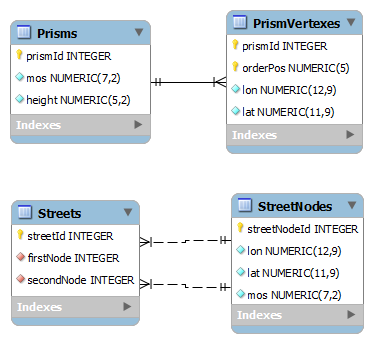
\includegraphics[width=25em]{img/static_db}
\end{center}
}
\par{
\begin{center}
\textit{Diagram ER bazy danych statycznych.}
\end{center}
}

\subsection{Baza danych dynamicznych}
\par{
Baza danych statycznych ma za zadanie zbierać informacje z czujników i stanowić element komunikujący symulator z dalszymi systemami bazującymi na jego wyjściu. Struktura tej bazy musi być w związku z tym możliwie elastyczna - by nie ograniczać przyszłego rozwoju całego ciągu narzędzi. Struktura ta została zaprojektowana we współpracy z twórcą oprogramowania korzystającego z wyników symulatora.
}
\subsubsection{Raport wykrycia}
\par{
Podstawowym pojęciem w przypadku bazy danych dynamicznych to \textit{raport o zauważeniu obiektu} (\textit{Detection Report}). Raport taki, zawiera w minimalnym przypadku współrzędne dokonanej obserwacji oraz jej czas. Jednakże, należy zwrócić uwagę, że ogólny projekt symulatora i całego ciągu narzędziowego dopuszcza możliwość dodawania do takiego raportu dodatkowych informacji w związku z czym baza musi posiadać dynamiczną strukturę, która umożliwia zapisanie tego rodzaju danych.
}
\par{
Zaproponowana struktura pozwala na łączenie każdego raportu wykrycia z dowolną ilością \textit{wartości dodatkowych} (\textit{Feature Value}). Wartość dodatkowa  zapisywana jest w postaci ciągu znaków którego interpretacja zależy od aplikacji, która dodatkowo może posiłkować się informacjami dotyczącymi typu danej - możliwej do uzyskania z opisu konkretnej wartości dodatkowej.
}
\par{
Każda wartość dodatkowa odnosi się bowiem do \textit{definicji wartości dodatkowej} (\textit(Feature for Sensor}). Tabela ta opisuje każdą klasę wartości dodatkowych typem informacji jaką za sobą ta klasa niesie oraz jej nazwą. Interpretacja znaczenia typu, który jest opisywany ciągiem znaków zależy od narzędzia docelowego, zakłada się jednak, że w typowym wypadku ciągi znaków będą zawierały nazwy typów zgodne z odpowiadającymi im typami w języku C++.
}
\subsubsection{Czujnik}
\par{
Innym elementem, który musi być opisany przez dynamiczną bazę danych by uniknąć niepotrzebnej zależności od bazy danych statycznych są czujniki. Każdy raport o zauważeniu obiektu musi posiadać informację na temat czujnika, z którego pochodzi - jest to kluczowa informacja dla analizy danych.
}
\par{
Podstawową informacją dotyczącą każdego czujnika jest jego położenie w przestrzeni oraz maksymalny zasięg. Maksymalny zasięg to odległość z jakiej dany czujnik może przy idealnych informacjach zebrać jakiekolwiek informacje.
}
\par{
Poza podstawowymi informacjami każdy czujnik może mieć swoją charakterystykę opisującą jego działanie (np. pole widzenia wyrażone w stopniach). Ponieważ typowo czujniki tego samego typu charakteryzują się podobnymi atrybutami, wprowadzono pojęcie typu opisywanego opcjonalnie nazwą. Każdy typ posiada zestaw atrybutów charakterystycznych dla siebie. Każdy atrybut posiada typ i opcjonalnie nazwę. Wiele czujników może wymagać takich samych informacji.
}
\par{
Dokładną strukturę bazy dynamicznej przedstawia poniższy diagram ER.
}


\par{
\begin{center}
\includegraphics[width=\textwidth,keepaspectratio]{img/dynamic_db}
\textit{Diagram ER bazy danych dynamicznych.}
\end{center}
}


\section[Architektura systemu][Architektura systemu]{Architektura systemu}
\par{
Zastosowanie poprawnej struktury architektonicznej całej aplikacji zdaje się mieć kluczowe znaczenie dla możliwości jej rozwoju, utrzymania jak i bezbłędnego napisania. Poprawna architektura chroni bowiem programistę przed jego własnymi błędami lub też pozwala na ich łatwe odnajdowanie.
}
\subsection{Model MVC}
\subsubsection{O modelu}
\par{
Model MVC (Model-View-Controller, z ang. Model-Widok-Kontroler) został zaproponowany jako całość w 1979 przez Trygve Reenskaug [19], choć --- co jest typowe dla wzorców projektowych --- był on wykorzystywany wcześniej niż został opisany. 
}
\par{
Model MVC dzieli aplikację lub jej część na trzy warstwy:
\begin{itemize}
\item \textbf{Model} - Model w założeniu stanowi element odpowiadający za przechowywanie i obróbkę danych na jakich pracuje dane oprogramowanie. Model posiada interfejs umożliwiający wykonywanie akcji na danych oraz dostęp do nich. Może, choć nie musi wykonywać akacje na danych niezależnie od wywołań z zewnątrz.
\item \textbf{Kontroler} - Zadaniem kontrolera jest przechowywanie kontekstu aplikacji, oraz przekazywanie zadań sterowania z widoku do modelu a także pobieranie z modelu informacji, których zażąda widok.
\item \textbf{Widok} - Widok odpowiada za prezentację danych użytkownikowi. Nie ma on świadomości procesów zachodzących na danych, zna jedynie sposób ich prezentacji oraz akcje jakie można na nich wykonać. Nie jest jednak świadom jak owe akcje wpłyną na te dane.
\end{itemize}
}
\par{
Podział taki zapewnia separację danych od sposobu ich prezentację co pozwala zbudować aplikacje o jednej funkcjonalności na wiele różnych sposobów z wieloma różnymi interfejsami utrzymując tylko jeden moduł odpowiedzialny za logikę aplikacji (model).
}
\subsubsection{Zastosowanie w aplikacji}
\par{
Model MVC zdawał się idealnie pasować do prezentowanego w pracy symulatora - posiada on bowiem całą funkcjonalność symulacji oraz zapisu danych, która jest całkowicie niezależna od sposobu prezentowania danych użytkownikowi. Brak jawnej separacji między modelem a interfejsem użytkownika zapewne doprowadził by do wymieszania tych warstw co mogło by spowodować między innymi następujące problemy:
\begin{itemize}
\item \textbf{Utworzenie zależności symulacji od działania intefrejsu - co prowadzi do braku możliwości prostej zamiany interfejsu w przyszłości.}
\item Rozsynchronizowanie stanu modelu z widokiem
\item Nieczytelność kodu spowodowana przeplataniem się kodu odpowiedzialnego za wyświetlanie danych i ich obsługę.
\end{itemize}
}
\subsection{Wielowątkowość}
\par{
Opisywany symulator został zaprojektowany by funkcjonować z wykorzystaniem trzech wątków:
\begin{itemize}
\item Odpowiedzialnego za obsługę modelu --- uruchamianego na początku symulacji i zmieniającego model wraz z upływem czasu.
\item Odpowiedzialnego za widok --- wątek główny przekazany jest we władanie biblioteki Qt, która uruchamia własną kolejkę komunikatów i w jej ramach obsługuje interfejs użytkownika.
\item Odpowiedzialnego za kontroler --- odpowiedzialny za przekazywanie informacji między widokiem a modelem.
\end{itemize} 
}
\subsubsection{Biblioteka boost::thread}
\par{
Do uruchamiania wątków wykorzystano przenośną bibliotkę boost::thread [20] umożliwiającą zaawansowane zarządzanie i synchronizację wątków. Biblioteka ta pozwoliła na łatwe uruchomienie wątków i zsynchronizowanie ich zakończenia. Pozwala ona bowiem na uruchomienie nowego wątku w oparciu o zadany obiekt-funktor [20] oraz zawieszenie dowolnego wątku posiadającego referencję do wątku na zawieszenie się w oczekiwaniu na jego zakończenie (join) [20]. Te funkcjonalności były wystarczające dla zastosowań projektu.
}
\par{
Biblioteka boost::thread została wybrana ponieważ jest dostępna dla wielu platform oraz nie wprowadza dodatkowych zależności (z tego powodu nie wybrano wątków dostarczanych przez bibliotekę Qt).
}

\subsubsection{Problemy synchronizacji}
\par{
Za każdym razem gdy aplikacja pracuje z wykorzystaniem więcej niż jednego wątku a między wątkami istnieje jakakolwiek forma komunikacji mamy do czynienia z problemami synchronizacji.
}
\par{
W przypadku opisywanego symulatora rozwiązaniem wszystkich problemów zdaje się być zwężenie wszelkiej komunikacji między-wątkowej do bezpiecznych wątkowo  kolejek komunikatów pozwalających na zawieszenie wątku w oczekiwaniu oczekiwanie na pojawienie się wiadomości. Dzięki ich zastosowaniu każdy wątek odbiera wiadomości w dogodnym dla siebie momencie i sam zmienia swoje dane --- jego dane zmieniane są tylko przez jeden wątek więc nie ma możliwości ich rozsynchronizowania.
\par{
Wadą takiego rozwiązania zdaje się być zwiększenia złożoności kodu ponieważ zamiast prostych wołań metod mamy do czynienia z dodawaniem wiadomości do kolejek. Z drugiej jednak strony dzięki temu wyraźnie widać w kodzie miejsca gdzie następuje komunikacja miedzy kluczowymi modułami aplikacji co ułatwia jego zrozumienie.
}


\section[Architektura modelu][Architektura modelu]{Architektura modelu}
\par{
Zaprojektowanie właściwej architektury modelu jest kluczowe dla celu tej pracy. Poprawnie zaprojektowany model powinien być możliwie elastyczny a jednocześnie pozwalać na szybkie zaimplementowanie minimalnego podzbioru funkcjonalności pozwalającego na uruchomienie symulacji.
}
\subsection{Obiekty świata}
\par{
Świat sam w sobie zna zasady fizyki opisane w wyżej wspomnianym modelu, nie wpływa jednak bezpośrednio na stan obiektów, które tym zasadom podlegają.
}
\par{
Obiekty wewnątrz modelu zdają się z łatwością dzielić na trzy grupy:
\begin{itemize}
\item Obiekty posiadające reprezentację fizyczną - np. budynki
\item Obiekty odbierające informacje o otoczeniu - np. czujniki
\item Obiekty posiadający obie powyższe właściwości - np. pojazdy
\end{itemize}
Z tego rodzaju podziału wyraźnie wynika możliwość podziału obiektów występującym w świecie na klasy - obserwatorów i obiekty o reprezentacji fizycznej, a także dziedziczące po obu obiekty żywe. Podział ten jest przedstawiony na poniższym fragmencie diagramu klas aplikacji.
}

\par{
\begin{center}
\includegraphics[width=30em]{img/obj_obs_cd}
\end{center}
}
\par{
\begin{center}
\textit{Podział obiektów na obserwatorów i fizyczne obiekty.}
\end{center}
}
\par{
Do zadań obserwatorów należy obsługa reakcji na zdarzenia nadchodzące z zewnątrz, obiekt natomiast ma za zadanie udostępniać wielkości fizyczne jakimi manipuluje autonomicznie obiekt --- siłę i masę.
}
\par{
Tylko obserwator jest świadom upływu czasu symulacji - może on zmieniać swój stan wraz z jego upływem. Obiekt nie posiada takiej możliwości - obsługa zmian jego stanu musi się odbywać przez interfejs obserwatora. W ten sposób obiekty statyczne nie będące obserwatorami automatycznie nie mogą zmieniać swojego stanu w czasie.
}
\par{
Obserwator otrzymuje wszelkie informacje w formie zrzutów z obiektów fizycznych. Zrzut zawiera nie więcej informacji niż posiada na temat obiektu świat (ponieważ jest przez świat tworzony), ale może zawierać ich mniej --- świat dobiera informacje przeznaczone dla poszczególnych obserwatorów.
}

\subsubsection{Wzorzec wizytatora}
\par{
Z punktu widzenia implementacji istotnym zdaje się być sposób zapewnienia obserwatorom możliwości obsługi poszczególnych rodzajów (typów) zrzutów z obiektów. Każdy z typów może być przecież traktowany osobno a sam typ jest już dla obserwatora rozpoznawalną informacją --- jeśli świat nie chciał by takiej informacji dostarczać nie tworzył by danego podtypu zrzutu.
}
\par{
Z pomocą w tej sytuacji przychodzi wzorzec wizytatora pozwalający obiektowi wchodzić w interakcje z obiektami z określonej hierarchii dziedziczenia w taki sposób by musiał on zapewnić specyficzną obsługę dla każdego jej podtypu.
}
\par{
W tym konkretnym zastosowaniu Obserwatorzy wizytują zrzuty i w ten sposób mogą ustawiać swój wewnętrzny stan i podejmować konkretne decyzje. W zależności od potrzeb Obserwator może albo reagować na kolejne wizytowane zrzuty lub podczas wizytacji zbierać informacje by podjąć decyzję po przejrzeniu wszystkich dostarczonych do niego danych.
}

\subsection{Upływ czasu}
\par{
W przypadku implementacji symulatora z modelem dynamicznym kluczowe jest poprawne i spójne obsłużenie upływu czasu dla modelu. W przypadku tej implementacji zastosowano powszechnie stosowaną w systemach czasu rzeczywistego architekturę żywej pętli. Architektura ta zapewnia możliwe wysoką precyzję przy odliczaniu czasu, jej niewątpliwą wadą jest natomiast nieoptymalne wykorzystanie zasobów.
}
\subsubsection{Biblioteka boost::chrono}
\par{
Inną od samej architektury kwestią jest zapewnienie spójnego systemu przeliczania czasu, szczególnie w kontekście czasu względnego względem realnego. Z pomocą przychodzi biblioteka boost::chrono [20] z zestawu bibliotek boost.
\par{
W chwili bieżącej biblioteka chrono jest elementem biblioteki standardowej języka C++, jednak w momencie rozpoczynania pracy nad aplikacją nie była ona jeszcze zbyt szeroko zaimplementowana w związku z tym zdecydowano się na jej pierwowzór - boost::chrono.
}
\par{
Biblioteka ta pozwala na wykonywanie wszelkich operacji związanych z czasem z uwzględnieniem spójności typów. Biblioteka rozróżnia moment w czasie, zakres czasów czy różnice w czasie jako odrębne typy i pozwala wykonywać na nich tylko takie operacje, które mają logiczny sens --- za każdym razem zwracając odpowiednio uzasadniony nowy typ.
}
\subsubsection{Wzorzec obserwatora}
\par{
Odrębną sprawą od samego przeliczania czasu jest fakt, że wiele obiektów w systemie powinno być w stanie reagować na upływ czasu w symulacji. Stworzono do tego celu interfejs SimulationPart (\textit{Element Symulacji} --- każdy element symulacji jest informowany gdy w symulacja posuwa się o kolejny krok.
}
\par{
Zastosowano to wzorzec obserwatora, gdzie wszystkie elementy symulacji (w tym w szczególności Obserwatorzy, którzy są elementami symulacji) obserwują symulację - symulacja powiadamia ich gdy upływa w niej pewien czas.
}

\subsection{Połączenie z bazą danych}
\par{
Istotnym elementem modelu symulatora jest komunikacja z bazą danych --- jest ona kluczowa zarówno dla inicjalizacji modelu jak i dla przekazywania jego wyjścia.
}
\subsubsection{Biblioteka pqxx}
\par{
Ponieważ wybrano silnik bazy danych postgreSQL należało odnaleźć możliwie obiektową bibliotekę z interfejsem w języku C++ pozwalającą na komuniakcję z taką bazą. Typowym rozwiązaniem jest zastosowanie biblioteki pqxx [22].
}
\par{
Biblioteka pqxx zapewnia spójny interfejs pozwalający na pełny dostęp do bazy postgreSQL na poziomie klienckim (tj. przy użyciu zapytań). Jest to funkcjonalność oczekiwana przez bibliotekę mającą zapewniać komunikację bazą w symulatorze.
}
\subsubsection{ORM}
\par{
ORM (ang. \textit{Object-Relational Mapping}, \textit{Mapowanie Obiektowo-Relacyjne}), to proces zamiany danych relacyjnych na dane obiektowe - typowy gdy chcemy wykorzystać relacyjną bazę danych do przechowywania danych na potrzeby aplikacji obiektowych.
}
\par{
Najprostsza zamiana krotek na obiekty polega na stworzeniu obiektów o strukturze identycznej ze strukturą krotki i przepisanie w odpowiednie atrybuty obiektu wartości pobranych z krotki. Również relacje typowo przekładalne są na wskaźniki lub referencje do odpowiednich obiektów klas powiązanych relacjami w bazie relacyjnej.
}
\par{
W przypadku opisywanej aplikacji takie mapowanie zdawało się być wystarczająco w związku z czym zbudowano bibliotekę pozwalającą na uzyskiwanie danych z RDBMS przy użyciu metod wykonujących odpowiednie zapytania a zwracających gotowe do dalszej pracy obiekty oczekiwane w pozostałych częściach aplikacji.
}

\subsection{Zarządzanie elementami symulacji}
\par{
Istotnym elementem symulacji jest tworzenie i usuwanie nowych obiektów --- elementów tejże symulacji. Do tego celu powołano klasę będącą podklasą elementu symulacji, mającą dostęp do wszystkich danych świata - który decyduje arbitralnie  wg. znanych sobie reguł o tworzeniu lub usuwaniu obiektów.
}
\par{
W przypadku przykładowej implementacji zarządca obiektów dodaje obiekty i usuwa je losowo gdy ich ilość w świecie jest różna od zadanej. Implementacja ta jest możliwie prosta - ponieważ pozwalała ona na szybkie uzyskanie działającej symulacji a dodanie do zarządcy większej logiki wymaga jedynie opisania właśnie tej logiki --- architektura pozwala na jego swobodną rozbudowę.
}

\subsection{Obsługa fizyki}
\par{
Świat jest klasą, która odpowiada za przekładnie akcji elementów symulacji na ich stan w świecie. Świat odbiera informacje o sile i masie od obiektów i na ich podstawie wyznacza ich przyśpieszenie a w konsekwencji chwilową prędkość.
}
\par{
Zadaniem świata jest również obsługa mapy jako że może ona wpływać na reakcje elementów symulacji.
}

\subsection{Komunikacja ze światem (API)}
\par{
Zadaniem głównej klasy modelu jest obsługa komunikacji z kontrolerem. W implementacji stanowiącej załącznik do tej pracy model udostępnia zewnętrznym modułom następujące operacje:
\begin{itemize}
\item Wystartuj symulację
\item Wstrzymaj symulację
\item Zatrzymaj symulację
\item Pobierz bieżący stan symulacji (zrzut)
\item Pobierz bieżący stan mapy (zrzut)
\item Pobierz bieżącą szybkość symulacji
\item Zmień szybkość symulacji na zadaną
\item Zarejestruj obserwatora stanu
\item Wyrejestruj obserwatora stanu
\end{itemize}
}
\subsubsection{Obserwacja stanu symulacji}
\par{
Zewnętrzne moduły mogą rejestrować się wewnątrz modelu jako obserwatorzy (w rozumieniu wzorca obserwatora) by być informowanymi o zmianach w modelu. Obserwator jest informowany za każdym razem, gdy model zmienia swój stan i tworzy nowe zrzuty mapy bądź obiektów w świecie. W typowym wypadku reakcją na taką notyfikację jest pobranie nowego stanu i jego wykorzystanie do swoich celów przez obserwatora.
}
\subsection{Kompletny diagram klas modelu}
\par{
\begin{center}
\includegraphics[width=\textwidth,keepaspectratio]{img/model_cd}
\end{center}
}

\section[Architektura widoku][Architektura widoku]{Architektura widoku}
\par{
Zadaniem widoku jest prezentowanie bieżącego stanu symulacji jak i udostępnienie odpowiednich kontrolek pozwalających sterować modelem.
}
\par{
Realizacja takiego zadania wymaga od biblioteki dwojakich możliwości - po pierwsze prezentacji w formie graficznej układu brył, czyli udostępnienie sceny dla wizualizacji 3D lub płótna dla wizualizacji 2D. Po drugie natomiast udostępnienia interaktywnych kontrolek pozwalających na wysyłanie do modelu określonych rozkazów. Biblioteka Qt zdaje się odpowiadać na obydwa te wymagania.
}
\subsection{Biblioteka Qt}
\par{
Podstawowym elementem biblioteki Qt jest zapewnienie synchronicznej i asynchronicznej komunikacji między wątkami jak i w ich obrębie za pomocą kolejki komunikatów obsługiwanej poza świadomością użytkownika.
}
\par{
Biblioteka ta, udostępnia mechanizm sygnałów i slotów jako interfejs pozwalający na łatwe korzystanie wyżej wspomnianego mechanizmu. Niestety ponieważ składniowo opis tego mechanizmu jest szerszy niż składnia języka C++, do jego tłumaczenia wykorzystywane jest dodatkowe narzędzie --- MOC (\textit{Meta-Object Compiler}).
}
\par{
Mechanizm ten pozwala jednak na szybkie definiowanie luźnych wiązań w obrębie modułów kontrolowanych przez bibliotekę Qt --- co jest niewątpliwie użyteczną cechą w przypadku interfejsów graficznych.
}
\subsubsection{QtGui}
\par{
Biblioteka QtGui pozwala na tworzenie interaktywnych formularzy z wykorzystaniem odpowiednich dla danej platformy metod --- typowo z wykorzystaniem natywnych kontrolek platformy. Głównym zadaniem tej biblioteki zdaje się być odcięcie logiki działania interfejsów graficznych od ich konkretnej implementacji. Dlatego ten sam kod wykorzystujący bibliotekę Qt skompilowany na różnych platformach daje inny kod wynikowy ale jednocześnie podobne odczucia użytkownika odnośnie interfejsu.
}
\subsubsection{QGraphicsLibrary}
\par{
QGraphicsLibary to biblioteka pozwalająca na definiowane 2.5 wymiarowych scen i wykonywanie na nich akcji logicznych a jednocześnie na bezpośrednie prezentowanie ich na ekranie w obrębie kontrolek biblioteki QtGui. Funkcjonalność ta zdawała się idealnie odpowiadać potrzebom wizualizacyjnym prezentowanej aplikacji i w związku z tym została ona wykorzystana do prezentowania użytkownikowi bieżącego stanu aplikacji.
}
\par{
Ponieważ widok jest obserwatorem stanu modelu, otrzymuje on informacje o jego nowym stanie i żąda nowych zrzutów kiedy uzna to za konieczne. Zrzut zawiera informacje na temat położenia, typu oraz innych atrybutów obiektu. W związku z tym, stosując ponownie wzorzec wizytora odpowiedni komponent widoku jest w stanie zmienić tę reprezentacje na odpowiadającą jej reprezentacje graficzną. Pozwala to na zachowanie kluczowej z punktu widzenia architektury aplikacji separacji między warstwami -- model nie ma żadnej informacji na temat sposobu prezentowania swojego stanu.
}

\section[Architektura kontrolera][Architektura kontrolera]{Architektura kontrolera}
\par{ 
Ostatnią warstwą modelu MVC, jest kontroler. Jego zadanie to przede wszystkim przekładanie zapytań widoku na operacje modelu oraz utrzymywanie stanu aplikacji.
}
\par{
Ponieważ zdecydowano się na uniknięcie integracji modelu z biblioteką Qt by nie wprowadzać trudnej do usunięcia zależności mechanizm sygnałów i slotów, choć pozwalający na niejawne budowanie bezpiecznych wątkowo kolejek komunikatów musiał zostać na etapie kontrolera zamieniony na typowe wołania języka C++.
}
\par{
Dodatkowym argumentem, który sugerował by tak postąpić był fakt, że praktyka pokazuje, że zastosowanie mechanizmów sygnałów i slotów, ze względu na brak jakichkolwiek ograniczeń w kwestii dodawania zdarzeń z dowolnego miejsca aplikacji - powoduje, że aplikacja przestaje bronić się przed próbami niezgodnego z architekturą przepływu informacji. Ponadto sygnały i sloty nie mają mechanizmów wykrywania błędów w czasie kompilacji - weryfikacja ich działania odbywa się dopiero w czasie działania aplikacji.
}
\par{
Odcięcie od mechanizmów Qt wykonano z wykorzystaniem prostego mechanizmu przekładania zdarzeń Qt na wiadomości pojawiającej się w kolejce komunikatów. Ostatnia klasa posiadająca zależność od biblioteki Qt, udostępnia odpowiednie dla wszystkich akcji możliwych do przekazania poza widok sloty. Obsługa każdego ze slotów tworzy na podstawie otrzymanych parametrów odpowiedni typ wiadomości i umieszcza tę wiadomość w kolejce komunikatów. Wątek kontrolera będący już niezależnym od biblioteki Qt wyjmuje kolejne wiadomości z tej kolejki i zapewnia im odpowiednią obsługę.
}